\section{Methods}


% what we did or tried to do
% define task to do and how we approached it
% explain pipeline and documentation and how to use it for posterity
% un annotated data, compared to

%\subsection{Development of the sleep staging pipeline} %??

\setcounter{subsection}{-1}
\subsection{Mathematical definitions}
\label{section:mathematical_definitions}
Before going further into the methods, it is relevant to make some mathematical definitions more clear and standardized regarding automatic sleep staging, extending the formalizations in section \ref{section:automatic_sleep_staging} and in \cite{Alexander2020}. 

% \begin{align}
%     \mathcal{S} = \{\textit{W, N1, N2, N3, REM}\} \\
%     y_k^{(i)} = \text{probability of sleep stage k at time step i} \rightarrow \mathbf{y} \in \mathbb{R}^{K \times N} \\
%     y^{\prime} \ _k^{(n)} = \frac{1}{\tau} \sum_{i=\tau(n-1)+1}^{\tau n} y_k^{(i)} = \text{ average probability of sleep stage k over the n-th window} \rightarrow \mathbf{y^{\prime}} \in \mathbb{R}^{K \times N/\tau} \\
%     s^{\prime} \ ^{(n)} = \mathcal{S}_{\argmax_{k} \left(y^{\prime} \ _k^{(n)} \right)} = \text{predicted label for the n-th window} \rightarrow \mathbf{s^{\prime}} \in \mathcal{S}^{N/\tau}
% \end{align}

First, the set of all possible sleep stages for each time step can be defined as the ordered list:
\begin{equation}
    \mathcal{S} = \{\textit{W, N1, N2, N3, REM}\}
\end{equation}

The number of possible labels, or possible sleep stages, $K$, is therefore always 5: $K = |\mathcal{S}| = 5$. The predicted sleep stage might also be reffered with $k$, with $k \in \mathbb{N} < 5$, and $\mathcal{S}_k$ corresponding to the $k$-th element in $\mathcal{S}$. Then, the probability of sleep stage $k$ at second $i$ is given by $y_k^{(i)}$, and all those probabilities aggregated in matrix format $\mathbf{y}$, with $N$ 1-second predictions in the data:
\begin{equation}
    y_k^{(i)} = \text{probability of sleep stage $k$ at second $i$} \rightarrow \mathbf{y} \in \mathbb{R}^{K \times N}
\end{equation}

We then perform the average of these probabilities for each class over each $\tau$ second window:
\begin{equation}
    y^{\prime} \ _k^{(n)} = \frac{1}{\tau} \sum_{i=\tau(n-1)+1}^{\tau n} y_k^{(i)} = \text{ average probability of sleep stage $k$ over the $n$-th window} \rightarrow \mathbf{y^{\prime}} \in \mathbb{R}^{K \times N/\tau}
\end{equation}

With this, the hypnogram is written as $\mathbf{S}$, and the predicted label for each second ($s^{\prime}$), is given by the $\argmax_k \left(y^{\prime} \ _k^{(n)} \right)$:
\begin{equation}
    s^{\prime} \ ^{(n)} = \mathcal{S}_{\argmax_{k} \left(y^{\prime} \ _k^{(n)} \right)} = \text{predicted label for the $n$-th window} \rightarrow \mathbf{S^{\prime}} \in \mathcal{S}^{N/\tau}
\end{equation}


%
%\subsection*{Analysis of predictions}




\subsection{Original pipeline} %==================================================================================
\label{section:original_pipeline}
As mentioned, most of the work on this project was built on top of a automatic deep learning sleep staging algorithm and pipeline developed in \cite{Alexander2020}. The algorithm was tested and validated on thousands of annotated sleep staging trials, from multiple cohorts, and trained in a number of different settings (like training with some cohort's data and validating on the others). Because the paper also provided the learned weights for the best model, these weights will be used for the predictions in our own data without much validation of their accuracy, especially because we lack annotated sleep staging data of our own to validate the model against.

% machine learning
The machine learning task at hand was to predict the sleep stage (wake, N1, N2, N3 or deep sleep, and REM sleep) of each 30 second window of time-dependent polysomnography (PSG) data. Because the data and the predictions are both time dependent, the goal was to infer, through machine learning, a function that could map PSG data to the corresponding sleep stage for that time window (or epoch).



\subsubsection{Network architecture}
The architecture of the network used in \cite{Alexander2020} was inspired by ResNet-50 \cite{olesen2018resnet} and adapted to 1-dimensional, time-dependent signals for classification tasks. A deep learning approach was used because it doesn't require preprocessing or manual feature extraction, and the mapping function is automaticly learned end to end.
An overview of the network architecture can be found in Fig.\ref{fig:network_architecture}. The training setup used the default parameter values of C = 4, $f_s = 128$ Hz, $T = \tau f_s$ , K = 5, R = 7, and $f_0 = 4$ for the number of input channels, sampling frequency, the sequence length, the number of sleep stages, the number of consecutive residual blocks, and the base filter kernel size,respectively, with $\tau$ being the number of successive 1 second predictions per epoch, usually just 30, but tested with other divisors of 30.


The network architecture essencially comprises:
\vspace{-0.3cm}
\begin{itemize}
    \item \textbf{A channel mixing module}, that changes the dimensions of the data to fit the latter part of the network, and introduces non-linear mixing between the channels' data.
    \item \textbf{A feature extraction module}, that comprises $R$ residual blocks, each using 2D convolutions to reduce the increase again the number of feature maps, batch normalizations and activations. Each block is simple, ensuring good conversion, and adding more blocks gives more expressivity to the network.
    \item \textbf{A temporal processing module}, that uses Gater Recurrent Units to introduce "past" and "future" dependencies on the data, mimicking how a human annotator would analyse the data.
    \item \textbf{A classification module}, that essencially performs a softmax activation on the results of the previous layer, giving the predicted probability of each sleep stage for each instant. The argmax of the results of the softmax for each instant give us the predicted stage of sleep for that instant.
\end{itemize}



\begin{figure}[H]
    \centering
    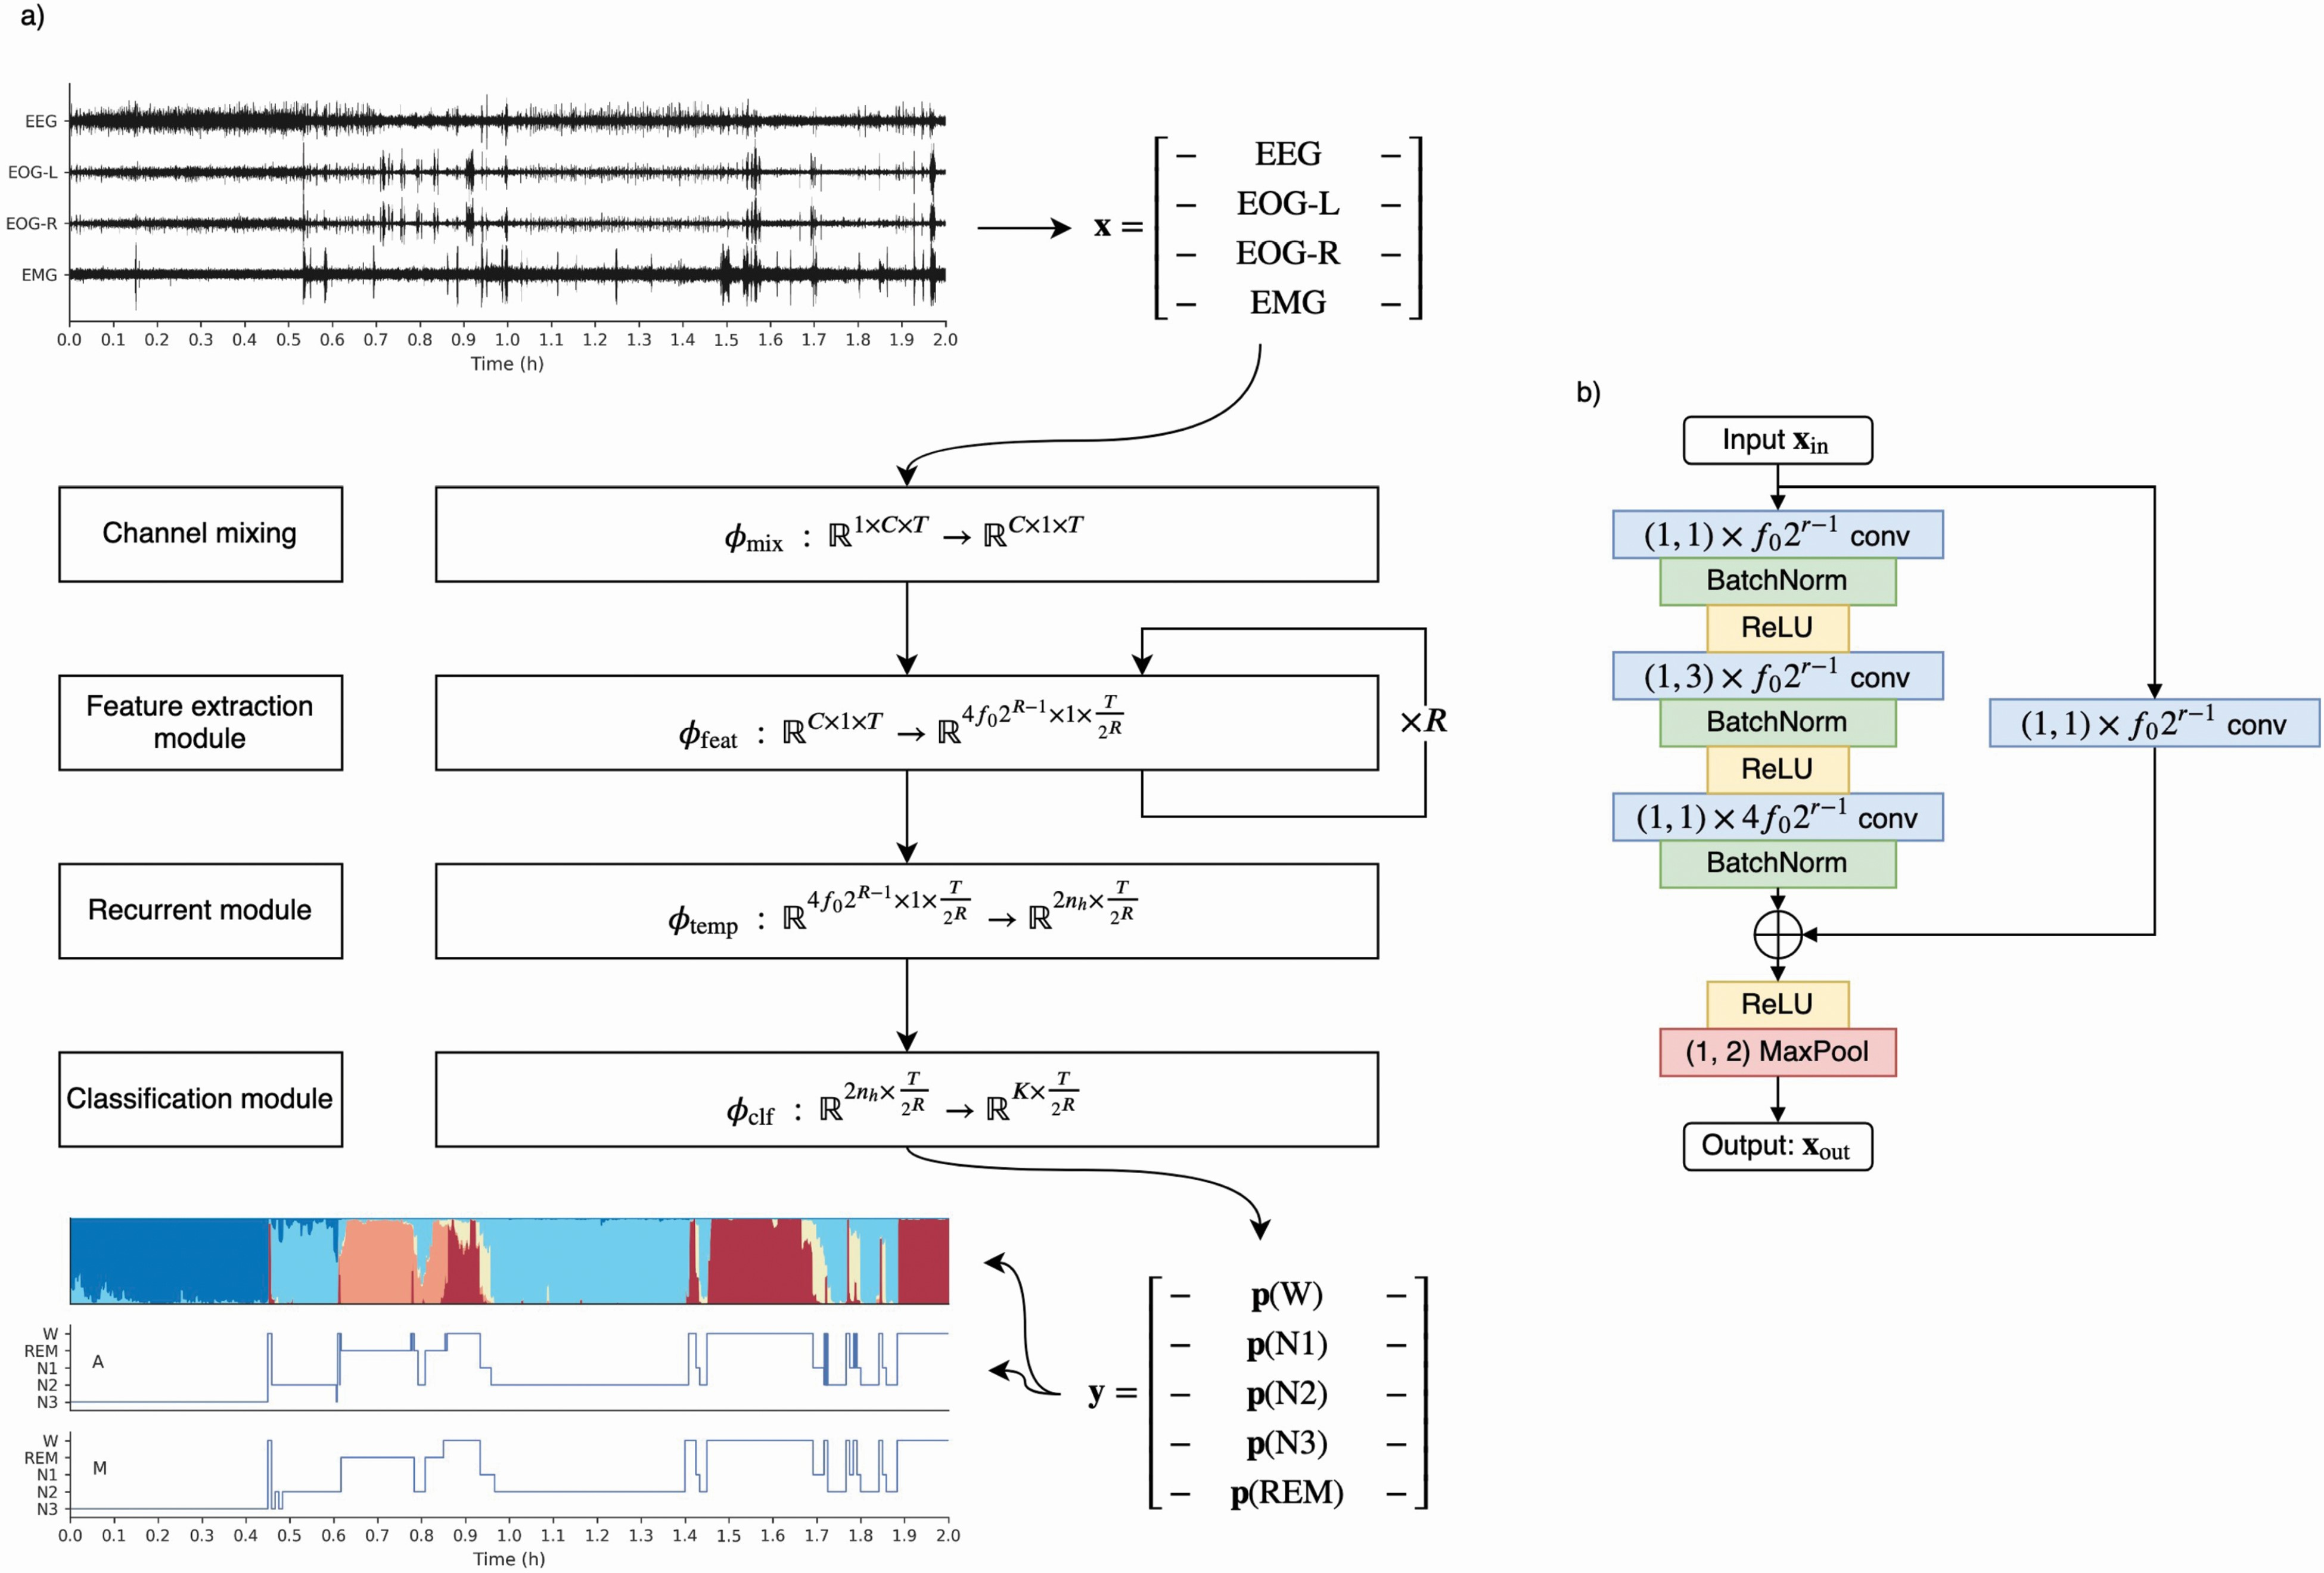
\includegraphics[width=0.8\linewidth]{Images/network_architecture.jpg}
    \caption{Network architecture used in \cite{Alexander2020}}
    \label{fig:network_architecture}
\end{figure}


\subsubsection{Steps of the pipeline}
A lot of the code used for this project, as well as the learned weights for the best model of the paper were made public though a GitHub repository \cite{Alexander2020}. Instructions on how and what to run in the pipeline are also available. Some essencial steps in the pipeline are:
\begin{itemize}
    \item \textbf{Setting up the PSG data .edf files} to be read in a folder and modify a config file to let the pipeline know the new location of the data. 
    \item \textbf{Latel identification}, by running a simple script that lets us map each electrode in our data to each electrode required by the pipeline, because there might not be a 1:1 correspondence between these.
    \item \textbf{Generate .h5 files from the data}, by running another script. Including modifying the code to extract the relevant patient metadata and data from our edf files. This step generates one h5 file for each subject, that includes the polysomnography data and ground truth hypnogram (if one was provided), as well as a .csv file for the cohort, with subject ID and file path information for each subject.
    \item \textbf{Inference on new data}, by calling the predict function with the learned weights on the h5 files, mentioning another config file. This generates .pkl files with the predicted sleep stage for each timestamp in the the PSG data, and performs some comparative metrics with the labeled hypnogram (if one was provided).
\end{itemize}



\subsection{Modifications to the pipeline} %===========================================================================
% Git hub and organization
The first step of coding for this project was to fork the original GitHub repository \cite{Alexander2020} to keep all of the original content while allowing to develop on top of that, keeping the coherence and structure The repository is available in \href{https://github.com/pplvieira/deep-sleep-pytorch-forked}{https://github.com/pplvieira/deep-sleep-pytorch-forked}. However some modifications had to be made on the code, and some envolved copying script files and hard coding some modifications on them, in order to fit some incompatibilities between the pipeline and our data and objectives for the project.
% LIBRARIES AND PYTHON VERSION
The scripts developed were run in the command line with Python 3.9.13, with notable libraries being matplotlib 3.7.1, yasa 0.6.5, scikit-learn 1.1.2 and pandas 2.1.0.

% Polysomnography
First, it is important to mention that the model was trained on polysomnography data. Meaning that it includes scalp EEG electrodes, as well as chin EMG and eletrooculogram (EOG). On the other hand, the data we have been acquiring is only from EEG channels.
Because of that, when mapping the channels from our data to the channels in the pipeline, the chin EMG and and EOG were left blanck, meaning that, after preprocessing of the channels, 1 out of the 4 data values that was passed to the model for each timestamp was zeroed out. 

% Lack of hypnogram
Another important incompatibility is that all throught the pipeline, it expects there to be a valid labeled hypnogram for the corresponding .edf file. However, the goal of this project was to perform predictions on new, unlabeled data, and comparing to the predictions from another pipeline to assess their agreement, not comparing with the ground truth (which was not available, as it would require a trained technician and a lot of time to annotate).
To work around this incompatibility with the pipeline, 2 of the python files were modified to \textbf{1:} produce a blank (all zeros) dummy hypnogram with the same size as the EEG data (instead of reading th hypnogram data from another .edf file) and \textbf{2:} ignore the comparison between predicted and "true" hypnogram at the end of the code, providing only the predictions, that would be compared to the results from other pipelines later.



\subsection{Additions to the pipeline} %===========================================================================
On top of the prediction pipeline, a few postprocessing and visualization scripts were made, to better visualize the results, manipulate the data and compare to other pipelines. These files, all located in a subfolder on the repository, are to be run as python scripts or modules, and include the \texttt{-h} flag and some other configurations to be called when running the code.

The scripts created are:
\vspace{-0.3cm}
\begin{itemize}
    \item \texttt{display\textunderscore hypnogram <predictionspath> --eval-window 30 --begining-index 0}: that simply manually retreives one predictions.pkl file (given in \texttt{predictionspath}) and plots the predicted hypnogram, as well as the distribution of the predicted relative probabilities of each sleep stage for each timestamp. The hypnogram is ploted using Yasa's \texttt{plot\_hypnogram} function \cite{2021yasa}.
    The eval-window can be change to perform averaging over the second-wise predictions in a smaller or larger window, the default, and most commonly used in the literature, is 30 (windows of 30 seconds). The time series of predictions is devided into chunks with size equal to the window size, and the predicted sleep stage for each chunk is the sleep stage with the highest probability inside all timestamps of that chunk of time. A larger window makes the output smoother but also loses time resolution. The begining index can also be changed, if, for example, the begining of the data corresponds to an awaken state, is too noisy or unpredictable and could be discraded for visualization.


    \item \texttt{predictions\textunderscore to\textunderscore txt --eval-window 30 --config <config>.yaml --prediction-dir \\ <predictdir> --output-dir <outputdir>}, which, for every file in the specified directory, converts the predictions.pkl into a .txt file in a lightweight and easy-to-read format, to be compared to other pipelines. This file format has one row for each epoch, with each row containing the predicted sleep stage. This step was included to make comparing results with other pipelines easier and streamlined, as the sleepEEGpy sleep staging wrapper \cite{belonosov2023sleepeegpy} exports the predicted hypnogram in this format. This function has a number of keyword arguments:
    \begin{itemize}
        \itemsep-0.4em
        \item \texttt{--eval-window}, that does the same as explained for the previous function (controling the size of each epoch), defaulted to 30.
        \item \texttt{--config}, references the .yaml file that was also used for obtaining the predictions in the original pipeline
        \item \texttt{--prediction-dir}, with the directory of all the .pkl predictions files, to be converted into the simple .txt format.
        \item \texttt{--output-dir}, with the directory of where the .txt files should be placed.
    \end{itemize}


    % dont know what im saying here
    \item \texttt{hypnogram\textunderscore comparison --folder <folderpath>}, which performs multi-rater analysis on multiple sleep staging predictions (from multiple different pipelines), each produced independently from the same .edf sleep EEG data. This function receives the folder of the .txt to be analyzed files as input. The .txt files presented can have different sizes (if for example 2 different window sizes were used for the same data), and the code will replicate the predictions of each file the number of times necessary for their duration to match (essencially make each file the size of the least common multiplier between their original sizes).
    %, but the sizes should be multiples of each other. 
    This script produces some plots:
    \begin{itemize}
        \itemsep-0.3em
        \item A confusion matrix for pairwise comparison of the predictions made by 2 of the raters for each timestep.
        \item A hypnogram comparison between which sleep stage each rater (each pipeline) has predicted for each time step, visualized as all hypnograms' time series superimposed as a function of time.
        \item A barplot with the proportion of number of agreers for each time stamp. Essencially telling, on how many timestamps do all the models agree.
        \item A matrix of inter-rater agreement (accuracy), essencially saying how much each pair of raters agree with each other (in case there are more than 2 raters).
        \item A matrix of inter-rater Cohen's kappa score, essencially the same as the previous, but with the Cohen's kappa instead of agreement.
    \end{itemize}
\end{itemize}

% mathematical defnitions of agreement and kappa
Using the notation from section \ref{section:mathematical_definitions}, given $M$ different raters (or different prediction pipelines) and $N$ epoch predictions from each, we want to define some metrics to compare the predictions between all of them. 
With $\mathbf{S^{\prime}}_{(l)}$ being the predicted hypnogram from rater $l$, we define $C^{(lm)}$ as the joint hypnogram between raters $l$ and $m$. I.e. $c_{ij}^{(lm)}$ is the number of epochs where rater $l$ predicts label $i$ and rater $m$ jointly predicts label $j$.

We then define agreement ($\text{Acc}^{(lm)}$) as the proportion of pairwise predictions that match between a pair of raters $l$ and $m$ (eq.\ref{eq:accuracy_definition}). 
\begin{equation}
    \text{Acc}^{(lm)} = \frac{\sum_{i} c_{ii}^{(lm)}}{\sum_{i,j} c_{ij}^{(lm)}}
    \label{eq:accuracy_definition}
\end{equation}
\vspace{-0.2cm}


Simillarly we define Cohen's kappa score between a pair of raters $l$ and $m$ ($\kappa^{(lm)}$), which takes into consideration the chance of the raters agreeing, and is a more robust measure of inter-rater reliability than accuracy. A kappa score of $\geq0.8$ is already considered almost perfect agreement. For $k$ categories, $N$ epochs to categorize and $n_{ki}$ the number of epochs where rater $i$ predicted category $k$:
\begin{equation}
    \kappa^{(lm)} = \frac{\text{Acc}^{(lm)} - p_e^{(lm)}}{1 - p_e^{(lm)}} \ , \quad p_e^{(lm)} = \frac{1}{N^2} \sum_{k} n_{kl} n_{km}
    \label{eq:kappa_definition}
\end{equation}
\vspace{-0.3cm}






\subsection{Pipeline features} % ??? %===========================================================================
\begin{figure}[H]
    \centering
    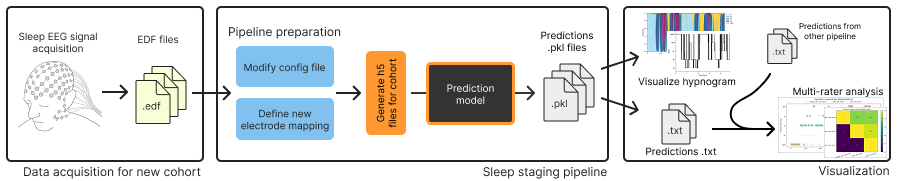
\includegraphics[width=1\linewidth]{Images/pipeline_diagram2.png}
    \caption{Simplified diagram of the full pipeline}
    \label{fig:pipeline_diagram}
\end{figure}
\vspace{-0.5cm}

% sequence + flexibility / tried to make it as readable as possible for the posterity
With this, we arrive at the final pipeline developed for this project, essencially consisting in a wrapper around the sleep staging pipeline in \cite{Alexander2020}. Fig.\ref{fig:pipeline_diagram} includes a schematic of the full pipeline. The 3 big blocks are essencially independent and almost isolated, and should be applied in sequence. Ensuring readability and ease of use for the posterity was also taken in consideration, in case automatic sleep staging continues to be of interest to Optoceutics and as more data is acquired through the years. 

% in more detail
The sleep data can be recorded through time with the protocol being used by Optoceutics and the research, and introduced into the pipeline as more and more data is gathered. The pipeline preparation steps only need to be done once for a new cohort of data, with cohort meaning a set of EEG .edf files with the same electrode setup and recording settings. As more data is introduced, generating the cohort files and passing them through the sleep staging prediction model is done by running 2 commands in the local terminal. The visualization part of the pipeline allows for manual visualization of the prediction results as well as small processing and comparison with the predictions from other pipelines, for a multi-rater assessment.

% what we can change (psg, swap model, compare to any prediction)
The parameters used on the pipeline preparation block for this project assumed the data consisted of a simple EEG recording, not a full polysomnography, to ensure consistency with the recordings we were provided. However, this results in loss of information, and most certainly in worse prediction results as well. If Optoceutics eventually acquires full polysomnography data, running the electrode mapping function again would ensure the information is not lost.
Aditionally, the prediction model is represented by a black box in the pipeline, as we are agnostic to the functioning of the model. It could also be swapped by another model as long as they take the same format of input and output. 
Finally, the multi-rater comparison can essencially be done with any number of other pipelines, as long they can be converted into the afformentioned .txt format. The analysis can also be done with manually labeled hypnograms if they are eventually obtained for Optoceutics' sleep recordings, meaning the prediction model or the data gathering could be validated. 

% COOPERATION + GOAL~~~
Finally, this project was done with a lot of colaboration from a collegue, who assessed the quality of another automatic sleep staging pipeline, using sleepEEGpy \cite{belonosov2023sleepeegpy}, a wrap around of another sleep staging Python library: YASA \cite{2021yasa}. The multi-rater analysis part of the pipeline developed here was mostly used to compare the results from each of the 2 pipelines, and because labeled sleep EEG data was unavailable, agreement between the raters was considered as a good enough proxi for the ground truth. In fact, as one the goal of the project was to expand Optoceutics' library of labeled sleep EEG data, and to assess the feasibility of further sleep studies, this multi-rater setup was more than enough.






